\documentclass{nature}

\usepackage[utf8]{inputenc}
\usepackage{graphicx}
\usepackage{amsmath}
\usepackage{amssymb}
\usepackage{booktabs}
\usepackage{multirow}
\usepackage{xcolor}
\usepackage{microtype}
\usepackage{float}
\usepackage[hidelinks]{hyperref}

\hypersetup{
  pdftitle={Stress-testing action transfer in an urban world model across four New York fare interventions},
  pdfauthor={AI Urban Scientist},
  pdfsubject={Retrospective leave-one-action-out evaluation of urban mobility forecasting},
  pdfkeywords={urban world model, action transfer, mobility forecasting, negative controls, New York City taxi}
}

\let\realincludegraphics\includegraphics
\AtBeginDocument{\let\includegraphics\realincludegraphics}
\makeatletter
\renewenvironment{figure}{\@float{figure}}{\end@float}
\renewenvironment{table}{\@float{table}}{\end@float}
\makeatother

\newcommand{\damgk}{DAM--GK}
\newcommand{\nmae}{\operatorname{NMAE}}

\begin{document}

\title{Stress-testing action transfer in an urban world model across four New York fare interventions}
\author{AI Urban Scientist}
\maketitle

\begin{abstract}
Urban forecasting models can fit recurring mobility patterns without learning how a city responds to an action. We test action transfer in a retrospective benchmark built from four official New York City yellow-taxi fare interventions, 263 taxi zones, 52 pre-action weeks and a sealed 12-week target window per action. Each outer fold trains on three actions and forecasts the fourth. A frozen action-conditioned geospatial residual model is compared with historical and spatial autoregression, a matched no-action model and seven corruptions of action timing, components and scope. Under the preregistered weeks 1/2/4/8/12 metric, correct-action error is 0.3684, compared with 0.3626 for History AR and 0.3614 for Spatial AR. The model improves two of four actions, passes none of eight transfer gates and is beaten overall by a four-week-delayed action. It loses both autoregressive baselines in six of seven fixed sensitivity specifications, but wins both when all 12 horizons are equally weighted. The benchmark therefore finds unstable, horizon-sensitive action transfer in this configuration, not a causal fare effect or a general failure of urban world models.
\end{abstract}

Forecasting mobility under an intervention is different from forecasting the next state of a familiar system. Graph-based traffic models capture spatial and temporal dependence well \cite{li2018dcrnn,yu2018stgcn,wu2019graphwavenet}, while world-model formulations make actions explicit in a learned transition system \cite{ha2018worldmodels}. Neither property alone shows that an action representation transports to an institutional change absent from fitting.

Traffic forecasting under shift is already a large field. Continual learning addresses evolving traffic networks \cite{chen2021trafficstream}; domain adaptation and graph transfer address changes across time, space and cities \cite{lu2021transfer,jin2023transgtr,deng2024domain}; and zero-shot traffic models target unseen urban regions \cite{li2025opencity}. These settings usually define an environment through geography, time or sensor topology. An official policy action adds declared timing, components and spatial applicability that can be changed independently at evaluation.

Event-aware mobility prediction is also established. Special-event models use nearby historical states \cite{yu2019specialevent}, while recent systems combine traffic with public-event text or semantic embeddings \cite{han2024eventtraffic,liang2024llmmpe,chen2025semob,yu2025fuse}. This work shows that event context can improve forecasts, but it does not answer whether a model trained on several policy actions prefers the correct semantics of a held-out action over plausible corruptions. The distinction matters because a model can respond to an action token while relying on date, event or exposure shortcuts.

We operationalize an urban world model as an action-conditioned geospatial forecasting system and test it with complete action-level holdouts. The paper makes four falsifiable contributions:
\begin{itemize}
\item a four-action benchmark in which each NYC fare intervention is an outer transfer environment and post-action targets are denied to model processes;
\item a tournament against strong historical dynamics, a matched no-action residual and seven frozen action corruptions;
\item event-, target- and horizon-level reporting that treats four actions, rather than 67,328 zone-week rows, as transfer support; and
\item a non-retuned sensitivity analysis that publishes a ranking reversal under equal weighting of all 12 horizons.
\end{itemize}

The frozen result is negative but structured. The evaluated configuration loses the primary comparison, improves the 2022 and 2025 actions while degrading the 2015 and 2019 actions, and fails to prefer correct action semantics consistently. Its conclusion also depends on horizon weighting. The scientific object is therefore the stress test and its falsification evidence, not a new graph architecture or a policy-effect estimate.

\section{Four actions define the transfer support}

The benchmark aligns four distinct fare actions to a common weekly state (Fig.~\ref{fig:design}a). The actions are the US\$0.30 citywide improvement surcharge effective 1 January 2015, the US\$2.50 congestion surcharge for applicable Manhattan trips effective 2 February 2019, the bundled TLC taximeter adjustment effective 19 December 2022, and the US\$0.75 Congestion Relief Zone taxi charge effective 5 January 2025 \cite{nys2019surcharge,tlc2022fare,mta2025crz}. Each event contains 52 complete pre-action weeks and 12 post-action weeks over the same 263 TLC Taxi Zones.

The observation table is large but the action design is small (Fig.~\ref{fig:design}b). Four events produce 67,328 zone-week rows; each outer fold fits 50,496 rows from three training actions. Zone-week replication measures within-event error precisely, but it does not create additional independent changes in policy timing or composition. We therefore weight events equally and report every held-out action.

Alongside the action-support counts in Fig.~\ref{fig:design}b, all 15 paper-level integrity checks pass. Runtime, evaluator and submission contracts were frozen before predictions; all 11 required submissions were committed; replay reproduced every fold without target access; and artifact hashes match the completion receipt. This establishes a completed model-held-out benchmark at the declared file boundary. It does not make the evaluation analyst-blind, because analysts had previously seen parts of the historical 2015 and 2025 periods.

\begin{figure}[H]
\centering
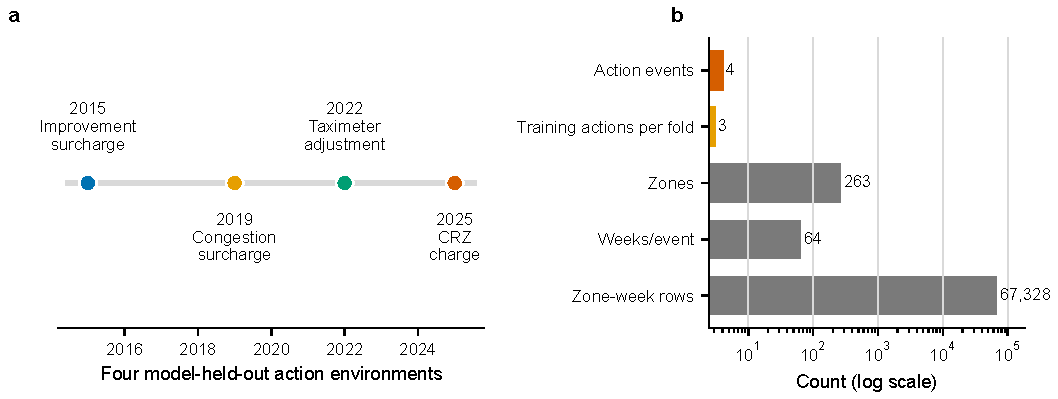
\includegraphics[width=\textwidth]{../figures/F1_benchmark_design.pdf}
\caption{\textbf{Four policy actions, not zone-week rows, define transfer support.} \textbf{a,} Timeline of the four model-held-out NYC yellow-taxi fare-action environments. \textbf{b,} Counts on a logarithmic scale. Each fold has only three training actions even though the complete panel contains 67,328 zone-week rows.}
\label{fig:design}
\end{figure}

\section{Correct action loses the frozen primary tournament}

Under the preregistered equal-event normalized mean absolute error, the correct-action model scores 0.368389 (Fig.~\ref{fig:primary}a). History AR scores 0.362616 and fixed-adjacency Spatial AR scores 0.361416, so the candidate errors are higher by 0.005773 and 0.006973, respectively. A matched residual network without action scores 0.372408. The architecture can change the backbone forecast, but the supplied action does not establish an advantage over simple historical dynamics.

The formal decision is stricter than a rank comparison (Fig.~\ref{fig:primary}b). The candidate has mean fold skill of $-2.52\%$ relative to History AR, improves two of four actions and passes 0/8 frozen gates. It misses the minimum mean skill, paired score interval, event-win, severe-loss, event-target, horizon, overall-control and fold-control criteria. Benchmark completion was independent of this decision, so the failed gate did not stop result emission.

The result supports a configuration-bounded statement (Fig.~\ref{fig:primary}a). The action-conditioned \damgk{} residual tested here does not transfer reliably under the frozen primary procedure. It does not support the broader statement that action conditioning, graph models or urban world models always fail.

\begin{figure}[H]
\centering
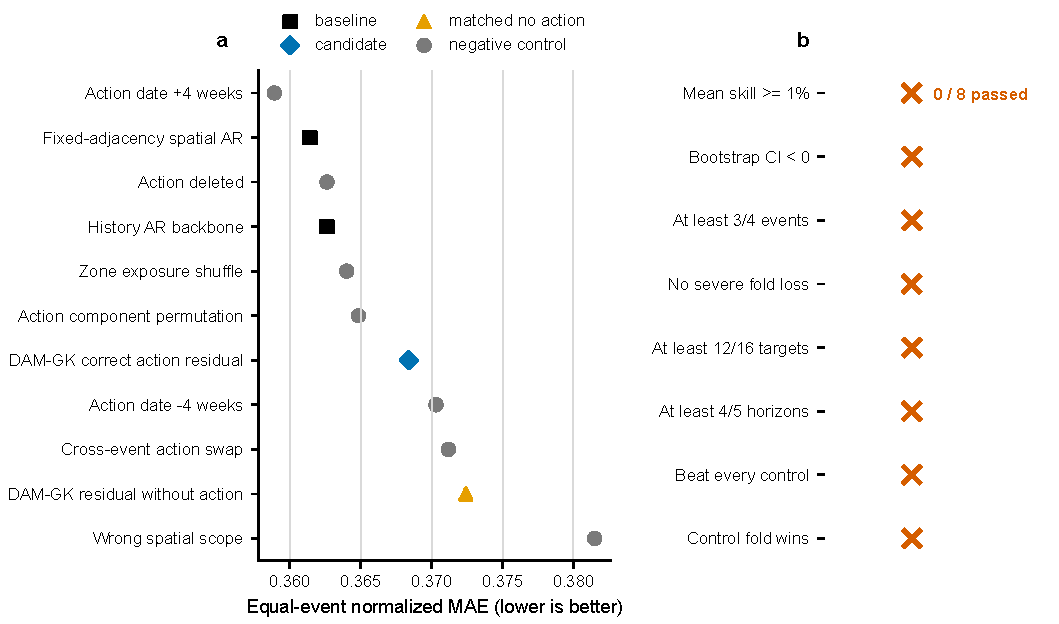
\includegraphics[width=\textwidth]{../figures/F2_primary_tournament.pdf}
\caption{\textbf{Correct action does not beat strong historical dynamics under the primary metric.} \textbf{a,} Equal-event pre-action-normalized MAE for the candidate, baselines, matched no-action model and seven frozen controls; lower is better. \textbf{b,} Outcomes of the eight preregistered transfer gates.}
\label{fig:primary}
\end{figure}

\begin{table}[H]
\caption{Primary equal-event model and control ranking.}
\label{tab:tab1_primary_scores}
\small
\begin{tabular}{rllr}
\toprule
Rank & Submission & Type & Error \\
\midrule
1 & Action date +4 weeks & negative control & 0.3589 \\
2 & Fixed-adjacency spatial AR & baseline & 0.3614 \\
3 & History AR backbone & baseline & 0.3626 \\
4 & Action deleted & negative control & 0.3626 \\
5 & Zone exposure shuffle & negative control & 0.3640 \\
6 & Action component permutation & negative control & 0.3648 \\
7 & DAM-GK correct action residual & candidate & 0.3684 \\
8 & Action date -4 weeks & negative control & 0.3703 \\
9 & Cross-event action swap & negative control & 0.3712 \\
10 & DAM-GK residual without action & matched no action & 0.3724 \\
11 & Wrong spatial scope & negative control & 0.3815 \\
\bottomrule
\end{tabular}
\end{table}


\section{Two actions improve and two degrade}

The mean hides a sharp event split (Fig.~\ref{fig:heterogeneity}a). Relative to History AR, candidate skill is $-15.35\%$ for the 2015 improvement surcharge and $-13.91\%$ for the 2019 congestion surcharge, but $+10.78\%$ for the 2022 taximeter adjustment and $+8.39\%$ for the 2025 CRZ charge. No single event explains the aggregate result, and a pooled trip-weighted score would answer a different question.

Target-level contrasts follow the same event partition (Fig.~\ref{fig:heterogeneity}b). All four targets worsen in 2015 and 2019 and improve in 2022 and 2025. Averaged across events, pickup error changes by only $-0.000118$, while drop-off, CBD inflow and CBD outflow errors increase by 0.008047, 0.008032 and 0.007130. The action residual is therefore neither uniformly inactive nor uniformly harmful.

These contrasts do not identify effects of the fare actions (Fig.~\ref{fig:heterogeneity}b). The four environments span different years, demand levels and concurrent conditions. Event heterogeneity is evidence about predictive transportability of this model, not about whether a surcharge increased or decreased taxi use.

\begin{figure}[H]
\centering
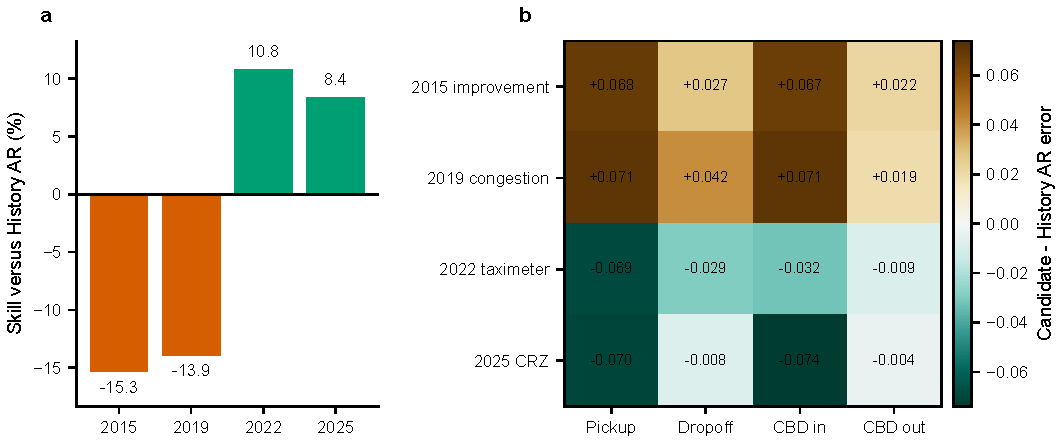
\includegraphics[width=\textwidth]{../figures/F3_event_heterogeneity.pdf}
\caption{\textbf{Transfer changes sign across actions and targets.} \textbf{a,} Skill of the correct-action candidate relative to History AR for each held-out action. Positive values favour the candidate. \textbf{b,} Candidate-minus-History AR error by event and target. Negative cells favour the candidate.}
\label{fig:heterogeneity}
\end{figure}

\begin{table}[H]
\caption{Leave-one-action-out skill relative to the History AR baseline.}
\label{tab:tab2_fold_skill}
\small
\begin{tabular}{lrrrrl}
\toprule
Held-out action & History AR & Correct action & Difference & Skill (\%) & Improves \\
\midrule
2015 improvement & 0.3010 & 0.3472 & 0.0462 & -15.3465 & No \\
2019 congestion & 0.3633 & 0.4138 & 0.0505 & -13.9118 & No \\
2022 taximeter & 0.3224 & 0.2877 & -0.0347 & 10.7765 & Yes \\
2025 CRZ & 0.4638 & 0.4249 & -0.0389 & 8.3861 & Yes \\
\bottomrule
\end{tabular}
\end{table}


\section{Semantic corruptions expose nonspecific action use}

Four of seven corrupted actions score better overall than the correct action (Fig.~\ref{fig:controls}a). Shifting the effective date four weeks later is the best submission in the full tournament, with error 0.358918. Correct action minus this control is $+0.009471$, and its paired taxi-zone bootstrap interval is $[0.005853,0.013101]$. Deleting the action, shuffling exposure and permuting components also produce lower overall error than correct action.

The candidate does reject some corruptions (Fig.~\ref{fig:controls}a). It beats the four-week-early date, cross-event action swap and wrong spatial scope overall. Yet no correct-versus-control comparison is won in all four folds, and fold-win counts range from one to three (Fig.~\ref{fig:controls}b). Correct semantics are therefore relevant in some comparisons but not reliably selected.

The delayed-date result is diagnostic, not an estimate of implementation lag (Fig.~\ref{fig:controls}a). A four-week shift may approximate adaptation, an omitted concurrent change or model misspecification. Because the control was frozen and not retuned after scoring, it shows that nominal timing was not identified consistently; it cannot establish that the real action began four weeks late.

\begin{figure}[H]
\centering
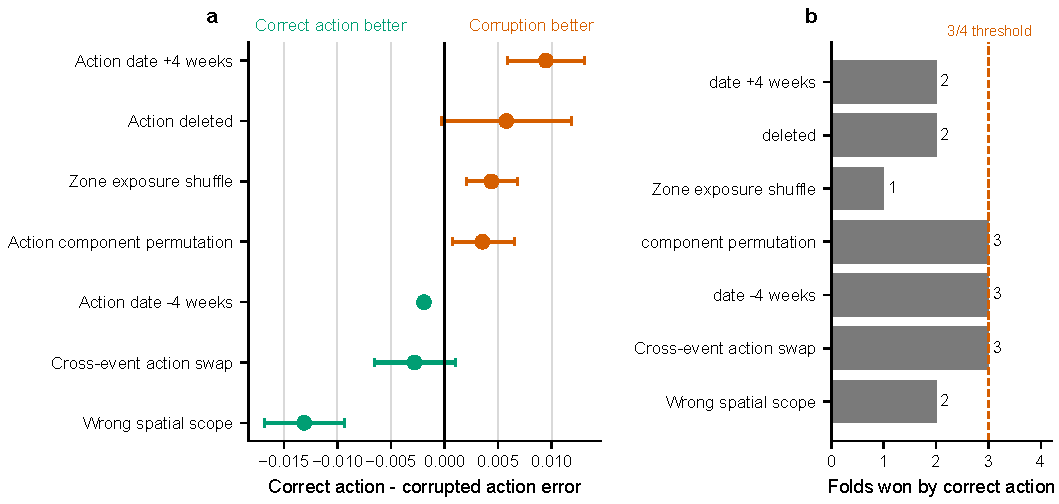
\includegraphics[width=\textwidth]{../figures/F4_semantic_controls.pdf}
\caption{\textbf{Correct action semantics are not reliably preferred.} \textbf{a,} Correct-action error minus each corrupted-action error with frozen 95\% paired taxi-zone bootstrap intervals. Negative values favour correct action. \textbf{b,} Number of the four outer folds won by correct action; the dashed line marks the required three-fold threshold.}
\label{fig:controls}
\end{figure}

\begin{table}[H]
\caption{Semantic action-control comparisons.}
\label{tab:tab3_action_controls}
\scriptsize
\setlength{\tabcolsep}{4pt}
\begin{tabular}{lrrrrr}
\toprule
Corrupted action & Error & Correct $-$ control & CI low & CI high & Fold wins \\
\midrule
Action date +4 weeks & 0.3589 & 0.0095 & 0.0059 & 0.0131 & 2 \\
Action deleted & 0.3626 & 0.0058 & -0.0003 & 0.0118 & 2 \\
Zone exposure shuffle & 0.3640 & 0.0044 & 0.0020 & 0.0068 & 1 \\
Action component permutation & 0.3648 & 0.0035 & 0.0007 & 0.0065 & 3 \\
Action date -4 weeks & 0.3703 & -0.0019 & -0.0022 & -0.0016 & 3 \\
Cross-event action swap & 0.3712 & -0.0028 & -0.0065 & 0.0010 & 3 \\
Wrong spatial scope & 0.3815 & -0.0131 & -0.0168 & -0.0093 & 2 \\
\bottomrule
\end{tabular}
\end{table}


\section{Horizon weighting changes the ranking}

The primary loss is concentrated at short horizons (Fig.~\ref{fig:sensitivity}a). Candidate-minus-History AR error is $+0.03736$ at week 1 and $+0.00587$ at week 2, but becomes negative at reported weeks 4, 8 and 12. Most unreported intermediate weeks also favour the candidate. Selecting weeks 1/2/4/8/12 therefore places more relative weight on the large week-1 miss than an equal mean across all 12 weeks.

The fixed sensitivity suite makes that dependence explicit (Fig.~\ref{fig:sensitivity}b). The candidate loses both autoregressive baselines under six of seven specifications, including log-MAE, median normalized absolute error, WAPE and minimum pre-event-scale restrictions. Under equal weighting of all 12 horizons, however, it scores 0.379255 versus 0.383750 for History AR and 0.383072 for Spatial AR, winning both comparisons. The preregistered failure is reproducible, but uniform inferiority across reasonable horizon weights is not supported.

Uncertainty has a second boundary (Fig.~\ref{fig:sensitivity}b). Frozen 20,000-draw paired bootstrap intervals are available for model-score differences. Calibrated predictive intervals are not: V5 retained scalar inner-fold validation metrics but not residual-level cross-fitted predictions for the training actions. Using the same held-out outcomes to calibrate intervals would leak test information, and variation across three random seeds measures ensemble spread rather than predictive coverage.

\begin{figure}[H]
\centering
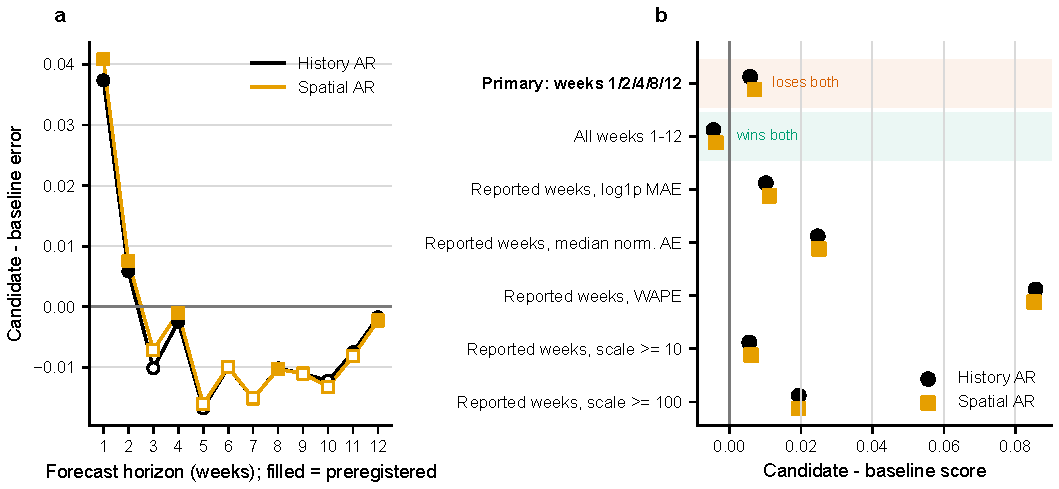
\includegraphics[width=\textwidth]{../figures/F5_horizon_metric_sensitivity.pdf}
\caption{\textbf{The transfer conclusion is sensitive to horizon weighting.} \textbf{a,} Candidate-minus-baseline normalized error for all 12 forecast weeks. Filled markers are the preregistered weeks 1, 2, 4, 8 and 12. \textbf{b,} Candidate-minus-baseline score for seven fixed, non-retuned specifications. The shaded rows place the primary metric beside the all-12-horizon reversal.}
\label{fig:sensitivity}
\end{figure}

\begin{table}[H]
\caption{Non-retuned metric and horizon sensitivity.}
\label{tab:tab4_metric_sensitivity}
\scriptsize
\begin{tabular}{llrrrrrl}
\toprule
Specification & Metric & Correct & History & Spatial & $\Delta$Hist. & $\Delta$Spatial & Outcome \\
\midrule
Reported weeks, all zones & Normalized MAE & 0.3684 & 0.3626 & 0.3614 & 0.0058 & 0.0070 & Loses both \\
All weeks 1--12 & Normalized MAE & 0.3793 & 0.3837 & 0.3831 & -0.0045 & -0.0038 & Wins both \\
Reported weeks, all zones & Log1p MAE & 0.2931 & 0.2829 & 0.2820 & 0.0102 & 0.0111 & Loses both \\
Reported weeks, all zones & Median normalized AE & 0.2179 & 0.1932 & 0.1929 & 0.0247 & 0.0250 & Loses both \\
Reported weeks, all zones & WAPE & 0.2105 & 0.1248 & 0.1253 & 0.0857 & 0.0852 & Loses both \\
Reported weeks, scale $\geq$ 10 & Normalized MAE & 0.2815 & 0.2760 & 0.2754 & 0.0055 & 0.0061 & Loses both \\
Reported weeks, scale $\geq$ 100 & Normalized MAE & 0.2218 & 0.2024 & 0.2025 & 0.0194 & 0.0194 & Loses both \\
\bottomrule
\end{tabular}
\end{table}


\section{Discussion}

This study asks a narrow question: does one action-conditioned geospatial model carry useful semantics from three documented fare actions to a fourth? Under the frozen primary metric, the answer is no. Strong autoregressive baselines perform better, only two events improve, and several semantically incorrect inputs outperform the official action. The result is more informative than a generic accuracy loss because the controls distinguish historical extrapolation, residual capacity and action specificity.

The benchmark also shows why action support must be counted at the event level. Tens of thousands of zone-week rows provide detailed measurements within four interventions, but each outer model still sees only three examples of how an institutional action differs. A spatially heterogeneous surcharge can add node-level exposure variation, yet it cannot replace independent changes in action composition. The partially supported inference is a design warning: row count should not be presented as policy-action sample size.

Horizon sensitivity changes how the negative result should be used. The candidate's large first-week miss drives the preregistered comparison, while intermediate horizons are generally favourable. One possibility is that the residual model represents slower adaptation better than immediate response. Another is that the apparent later advantage reflects shared temporal structure rather than action semantics, consistent with the control failures. The current benchmark separates these explanations imperfectly; future protocols should declare operational horizon weights from the use case and retain all horizons for secondary reporting.

Four limitations bound the evidence. First, the benchmark contains only four NYC yellow-taxi actions and no independent city. Second, it is model-held-out but not analyst-blind, and a genuinely prospective V6 event has not been activated. Third, cross-year shocks and changes in taxi reporting prevent causal interpretation. Fourth, calibrated predictive intervals cannot be reconstructed from retained V5 artifacts. None of these limitations invalidates the frozen score comparison, but each restricts the claim it can support.

The next empirical step is not to tune V5 after observing its failures. It is to retain cross-fitted residual predictions, predeclare horizon utilities, and evaluate a genuinely future action once its outcome window closes. A stronger benchmark would add cities and policies with independently varying timing, magnitude and spatial scope. Until then, the appropriate conclusion is that action transfer in this evaluated configuration is unstable and horizon-weighting sensitive.

\begin{methods}

\subsection{Study design and scope}

The study is a retrospective leave-one-action-out predictive benchmark. The independent transfer environments are four NYC yellow-taxi fare actions in 2015, 2019, 2022 and 2025. Each outer fold uses three actions for fitting and nested selection, supplies the fourth action's 52 pre-action weeks as history and graph input, and denies all 12 post-action target weeks to model processes. The inferential target is predictive transportability of one frozen configuration across these actions. No causal, welfare, congestion-reduction, cross-city or operational claim is made.

\subsection{Mobility data and spatial units}

Weekly state derives from official NYC TLC Yellow Taxi trip records and the 263-zone TLC Taxi Zone system \cite{tlctripdata}. The four targets are pickup count, drop-off count, CBD inflow attributed to origin zone and CBD outflow attributed to destination zone. The benchmark consumes the retained event panels named \path{heldout_2015_event_panel.parquet} and \path{development_event_panel.parquet}, plus daily origin--destination panels for pre-action graph construction. Their full workspace paths and hashes are recorded in \path{results/evidence_inventory.csv}. Each event forms a complete $64\times263$ weekly grid. Missing zone-weeks enter as declared zeros only after source admission and completeness checks in the upstream panel builders.

The four event windows are 2 January--31 December 2014 plus 1 January--25 March 2015; 3 February 2018--1 February 2019 plus 2 February--26 April 2019; 20 December 2021--18 December 2022 plus 19 December 2022--12 March 2023; and 7 January 2024--4 January 2025 plus 5 January--29 March 2025. Weeks are complete seven-day blocks aligned to each effective date.

\subsection{Action representation and official evidence}

Each zone-week has 15 numeric action features. Ten encode expected per-trip contributions for fixed spatial surcharge, flag fall, improvement surcharge, metered unit, rush hour, night, JFK flat fare, JFK rush, LaGuardia and Newark terms. Five encode expected total and fractional fare change, spatial applicability, temporal applicability and implementation share. Event name, year, policy name and outer-fold identity are forbidden model features.

Official evidence fixes the action dates and values. New York State guidance documents the 2019 surcharge \cite{nys2019surcharge}; the adopted TLC fare rule documents the 2015 improvement surcharge and the bundled 2022 taximeter changes \cite{tlc2022fare}; and the MTA schedule documents the 2025 CRZ taxi charge \cite{mta2025crz}. These sources define predictive inputs. They are not used as causal instruments.

\subsection{Spatial relations}

Each fold contains three relations. Geographic adjacency is frozen from TLC zone polygons. Origin--destination flow retains the eight largest non-self outgoing destinations per origin, using only that event's 52 pre-action weeks. Action exposure is a self relation carrying the frozen numeric exposure for each zone. Relation weights are row-normalized. No post-action target or post-action graph update is permitted for the held-out event.

\subsection{Historical baselines}

History AR models log-count residuals relative to the mean log state over the 52 pre-action weeks. Separate ridge models are fit for every zone with lags 1, 2, 4 and 8 and fixed regularization 5.0. Calendar inputs encode annual phase, clipped event-relative time, a post-action flag and an intercept. Forecasts are rolled recursively for 12 weeks. Spatial AR adds the geographic-adjacency message from lag 1 but otherwise uses the same construction.

\subsection{Action-conditioned residual model}

The candidate predicts a residual correction to the committed History AR forecast,
\begin{equation}
\widehat y^{\mathrm{candidate}}_{e,z,h,k}
=\widehat y^{\mathrm{history}}_{e,z,h,k}
+s_{e,z,k}\,f_{\theta}(x_{e,z,h},m_{e,z,h},c_{e,h},a_{e,z,h}),
\end{equation}
where $e,z,h,k$ index event, zone, horizon and target; $s$ is the pre-action zone-target mean clipped below at one; $x$ contains the backbone forecast, final pre-action state and four-week trend; $m$ contains messages from the three relations; $c$ contains calendar and horizon phase; and $a$ is the scaled 15-feature action.

The neural residual uses an eight-dimensional node embedding, a two-layer state encoder, a 15-to-16-dimensional action encoder and a two-layer four-target head. The final head is initialized at zero. For action-conditioned variants, a zero action masks the predicted residual to zero, providing an architectural zero-action anchor. Compact, base and regularized configurations differ in hidden width, learning rate, weight decay and training epochs.

Within each outer fold, the three training actions are rotated through inner leave-one-action-out selection. The selected configuration is refit on all three actions for seeds 31, 47 and 73. Predictions are averaged in raw count space after every seed emits the complete key set. Forecasting is open-loop for 12 weeks and does not write observed test states back into the model.

\subsection{Matched model and semantic controls}

The matched no-action model retains the backbone and residual architecture but removes action inputs. Seven frozen controls alter one declared semantic aspect: delete the action, shift the effective date four weeks earlier or later, permute the ten fee components, assign the wrong spatial scope, swap the action across events, or shuffle zone exposure with seed 20260723. All controls use identical folds, keys, seed requirements and evaluation code. They are predictive falsification controls, not estimates of causal counterfactuals.

\subsection{Primary metric and decision rule}

For event $e$, zone $z$ and target $k$, the error scale is the target's mean over 52 pre-action weeks, clipped below at one. For the reported horizons $H=\{1,2,4,8,12\}$,
\begin{equation}
E_e=\frac{1}{|Z||K||H|}
\sum_{z\in Z}\sum_{k\in K}\sum_{h\in H}
\frac{|\widehat y_{e,z,h,k}-y_{e,z,h,k}|}
{\max(\overline y^{\mathrm{pre}}_{e,z,k},1)},
\qquad E=\frac{1}{4}\sum_e E_e.
\end{equation}
Fold skill against History AR is $1-E_e^{\mathrm{candidate}}/E_e^{\mathrm{history}}$.

The all-required transfer gate tests mean skill of at least 1\%, a paired score-difference interval entirely below zero, improvement in at least three events, no event degradation beyond 2\%, improvement in at least 12 of 16 event-target cells and four of five reported horizons, and superiority to every semantic control overall and in at least three folds. Benchmark completion does not require a passing model.

\subsection{Score uncertainty and sensitivity}

Paired uncertainty is computed at the taxi-zone level within each event. Normalized candidate-minus-baseline errors are averaged within each event-zone, zones are resampled with replacement 20,000 times using seed 20260723, and the four event means receive equal weight. Percentile intervals describe uncertainty in a score difference conditional on these four events; they do not represent a population of policies.

Seven non-retuned sensitivity specifications reuse the committed predictions. They compare the primary normalized MAE, median normalized absolute error, log1p MAE and WAPE on reported horizons; normalized MAE over all 12 horizons; and normalized MAE after minimum pre-event target scales of 10 and 100. No specification changes model fitting or the frozen gate.

Calibrated predictive intervals were audited but not constructed. The retained artifacts contain scalar inner-fold validation metrics rather than residual-level cross-fitted training-action predictions. Calibrating on the same held-out action targets used for scoring would violate the fold firewall. Three-seed variation is therefore not reported as interval coverage.

\subsection{Commitment, replay and reproducibility}

The suite protocol, Runtime-R4 contract, evaluator and submission contract were sealed before formal prediction. Each model process was denied the current outer fold's post-action target path and other submissions for that fold. All model, control, seed and fold artifacts were committed before evaluator access, then replayed and hash-checked. The frozen evaluator emitted a result regardless of gate outcome.

Authoritative paper inputs are listed in \path{results/evidence_inventory.csv}. Experiment scripts are in the adjacent \path{exp/} directory; extracted results, figure source CSVs and LaTeX tables are stored beside the manuscript. No public code URL is asserted. The separate global Chongqing data-seeker report is not used by this NYC study.

\subsection{Data availability}

TLC trip records and Taxi Zone resources are available from the official TLC archive \cite{tlctripdata}. Fare-action documents are public official records \cite{nys2019surcharge,tlc2022fare,mta2025crz}. Frozen local manifests and completion receipts record file paths, sizes and SHA-256 hashes. Derived weekly panels and committed predictions are retained in the project workspace. This study uses no synthetic mobility observations.

\end{methods}

\begin{addendum}
\item[Competing interests] The author declares no competing interests.
\end{addendum}

\bibliographystyle{naturemag}
\bibliography{references}

\end{document}
